\section{Fensterfunktionen}
Eine wichtige Funktion der Stream Analytics-Abfragesprache SAQL ist die Möglichkeit, mit Zeitfenstern zu arbeiten. Ergebnisse werden mithilfe dieser Funktion entsprechend gruppiert. Dies ist vergleichbar mit der GROUP BY-Klausel von SQL mit einer der folgenden Erweiterungen:
\begin{itemize}
\item Azure-Blobspeicher 
\item TumblingWindow
\item HoppingWindow
\item SlidingWindow
\end{itemize}
Beispielsweise soll nun eine Abfrage gestartet werden. Diese soll aufzeigen, wie viele Autos einer speziellen Farbe alle fünf Minuten eine Mautstelle passieren. Mit TumblingWindow kann diese Abfrage so 1:1 implementiert werden. Bei HoppingWindow lässt sich zwar die gleiche Abfrage ausdrücken, allerdings kann hier unabhängig von der Fenstergröße eine Ausgabe erzeugt werden. Es könnte hier beispielsweise einmal pro Minute ausgegeben werden, wie viele Autos einer speziellen Farbe alle fünf Minuten diese Mautstelle anfahren. SlidingWindow hingegen lässt die Abfrage zu, in welchen 5-Minuten-Zeitfenstern zehn oder mehr Autos einer speziellen Farbe die Mautstelle erreichen. SlidingWindow ist somit für den Umgang mit relativ spärlichen Ergebnismengen geeignet. Diese Konzepte sind in Abbildung \ref{fig:window_concepts} dargestellt [6].\\ \\

\begin{figure}[h!]
	\centering
	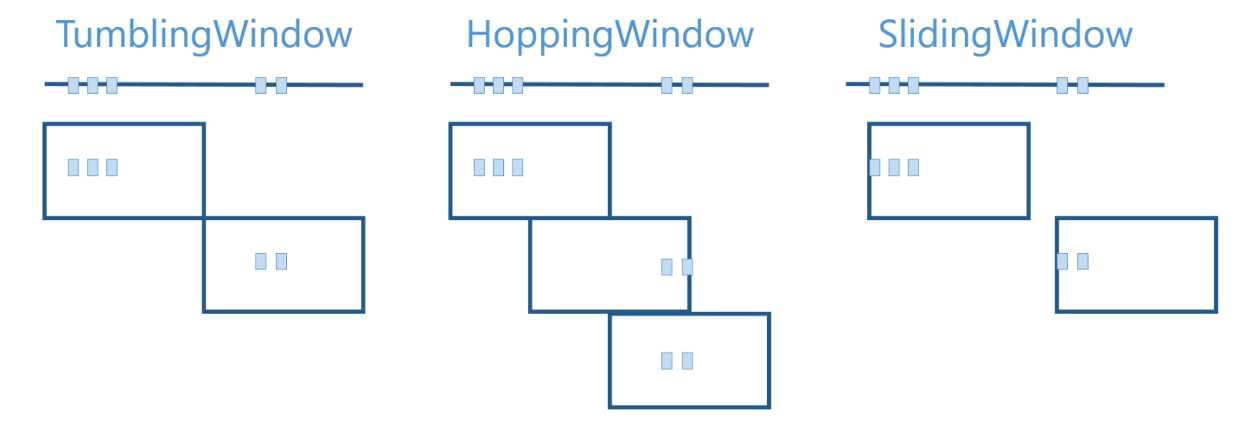
\includegraphics[width=1.0\linewidth]{images/fensterfunktionen}
	\caption{Fensterkonzepte} %Generelle
	\label{fig:window_concepts}
\end{figure}
